\documentclass{beamer}
\usetheme{Madrid}
\usecolortheme{default}

\usepackage[utf8]{inputenc}
\usepackage{graphicx}
\usepackage{tikz}
\usetikzlibrary{shapes,arrows,positioning,fit,backgrounds}
\usepackage{listings}
\usepackage{algorithm}
\usepackage{algpseudocode}
\usepackage{pdflscape}
\usepackage{amsmath}

% Path to images (relative to this file)
\graphicspath{{../report/images/}}

\title[EHR: Pharmacy Module]{Electronic Health Record: Pharmacy Organization Module}
\subtitle{Enterprise-Grade Platform Using Hyperledger Fabric and Docker Swarm}
\author[Ankit, Mohit, Ronit]{
    ANKIT CHAUDHARI (25CSM2R03) \\
    MOHIT TOMAR (25CSM2R13) \\
    RONITSINGH RAWAT (25CSM2S06)
}
\institute[NITW]{
    Under the guidance of \textbf{PROF. ERUKALA SURESH BABU} \\
    \vspace{10pt}
    DEPARTMENT OF COMPUTER SCIENCE AND ENGINEERING \\
    NATIONAL INSTITUTE OF TECHNOLOGY WARANGAL
}
\date{April, 2026}

\begin{document}

\begin{frame}
    \titlepage
\end{frame}

\begin{frame}{Outline}
    \tableofcontents
\end{frame}

\section{Introduction}
\begin{frame}{Abstract}
    The Electronic Health Record (EHR) System is a decentralized, secure, and scalable platform designed for pharmaceutical inventory and patient record management.
    \begin{itemize}
        \item \textbf{Decentralization:} Built on Hyperledger Fabric.
        \item \textbf{Privacy:} Attribute-Based Access Control (ABAC).
        \item \textbf{Scalability:} Docker Swarm orchestration across multiple nodes.
        \item \textbf{Hybrid Storage:} On-chain metadata and off-chain IPFS document storage.
    \end{itemize}
\end{frame}

\section{System Architecture}
\begin{frame}{High-Level Architecture}
    \centering
    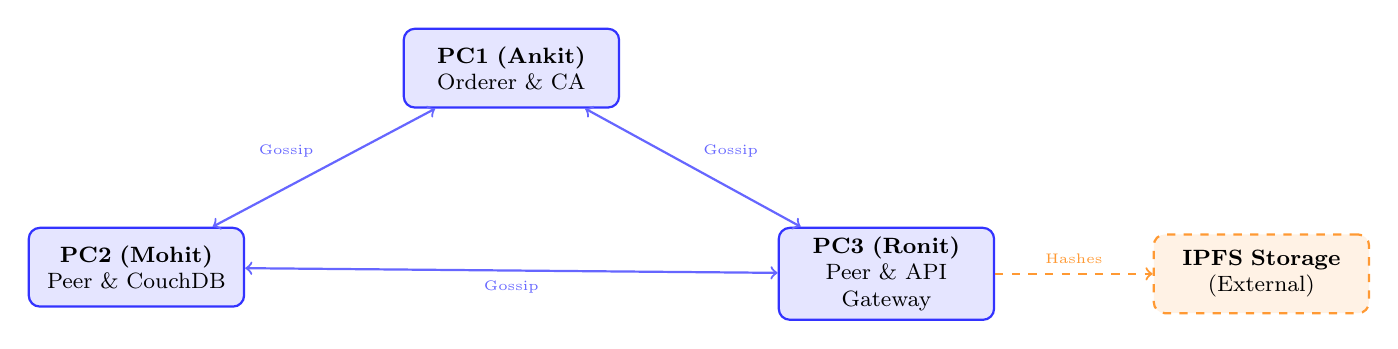
\begin{tikzpicture}[
        node distance=1.5cm and 2cm,
        box/.style={draw=blue!80, fill=blue!10, text width=2.5cm, align=center, minimum height=1cm, rounded corners, thick, font=\footnotesize},
        ext/.style={draw=orange!80, fill=orange!10, text width=2.5cm, align=center, minimum height=1cm, rounded corners, thick, dashed, font=\footnotesize}
    ]
        
        \node[box] (pc1) {\textbf{PC1 (Ankit)}\\Orderer \& CA};
        \node[box, below left=of pc1] (pc2) {\textbf{PC2 (Mohit)}\\Peer \& CouchDB};
        \node[box, below right=of pc1] (pc3) {\textbf{PC3 (Ronit)}\\Peer \& API Gateway};
        
        \node[ext, right=2cm of pc3] (ipfs) {\textbf{IPFS Storage}\\(External)};
        
        \draw[<->, thick, blue!60] (pc1) -- node[above left, font=\tiny] {Gossip} (pc2);
        \draw[<->, thick, blue!60] (pc1) -- node[above right, font=\tiny] {Gossip} (pc3);
        \draw[<->, thick, blue!60] (pc2) -- node[below, font=\tiny] {Gossip} (pc3);
        
        \draw[->, thick, dashed, orange!80] (pc3) -- node[above, font=\tiny] {Hashes} (ipfs);
        
    \end{tikzpicture}
    \vspace{10pt}
    \begin{itemize}
        \item Layered Tiers: Presentation, Application, Blockchain, Storage.
        \item Distributed over 3 physical machines via Tailscale VPN.
    \end{itemize}
\end{frame}

\begin{frame}{Transaction Flow: Write Operation}
    \centering
    \scalebox{0.55}{
    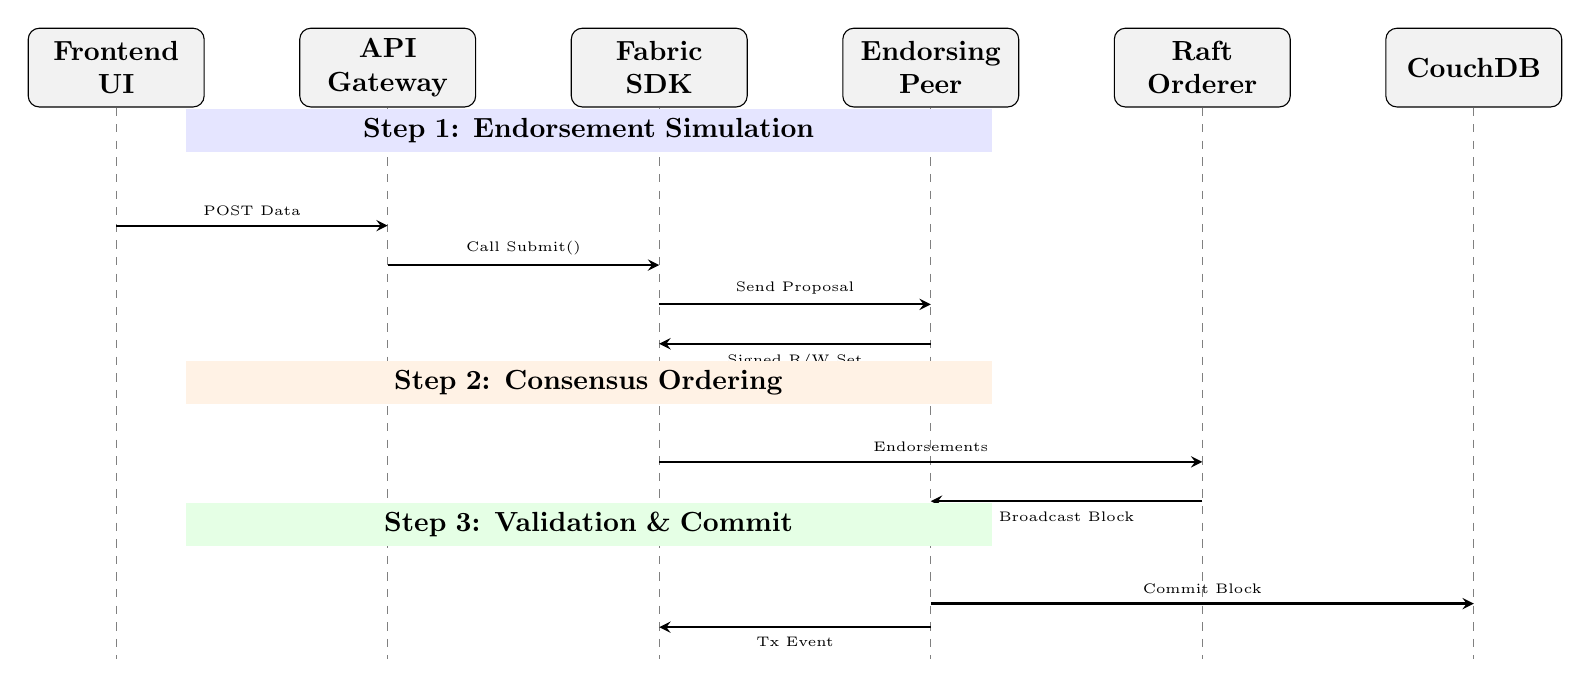
\begin{tikzpicture}[
        node distance=1.2cm,
        actor/.style={draw, fill=gray!10, text width=2cm, align=center, minimum height=1cm, rounded corners},
        arrow/.style={->, thick, >=stealth}
    ]
        \node[actor] (UI) {\textbf{Frontend UI}};
        \node[actor, right=of UI] (API) {\textbf{API Gateway}};
        \node[actor, right=of API] (SDK) {\textbf{Fabric SDK}};
        \node[actor, right=of SDK] (Peer) {\textbf{Endorsing Peer}};
        \node[actor, right=of Peer] (Orderer) {\textbf{Raft Orderer}};
        \node[actor, right=of Orderer] (DB) {\textbf{CouchDB}};

        \foreach \i in {UI, API, SDK, Peer, Orderer, DB} {
            \draw[dashed, gray] (\i.south) -- ++(0,-7);
        }
        
        \node[fill=blue!10, text width=10cm, align=center] at (6,-0.8) {\textbf{Step 1: Endorsement Simulation}};
        \draw[arrow] ([yshift=-1.5cm]UI.south) -- node[above, font=\tiny] {POST Data} ([yshift=-1.5cm]API.south);
        \draw[arrow] ([yshift=-2.0cm]API.south) -- node[above, font=\tiny] {Call Submit()} ([yshift=-2.0cm]SDK.south);
        \draw[arrow] ([yshift=-2.5cm]SDK.south) -- node[above, font=\tiny] {Send Proposal} ([yshift=-2.5cm]Peer.south);
        \draw[arrow] ([yshift=-3.0cm]Peer.south) -- node[below, font=\tiny] {Signed R/W Set} ([yshift=-3.0cm]SDK.south);
        
        \node[fill=orange!10, text width=10cm, align=center] at (6,-4.0) {\textbf{Step 2: Consensus Ordering}};
        \draw[arrow] ([yshift=-4.5cm]SDK.south) -- node[above, font=\tiny] {Endorsements} ([yshift=-4.5cm]Orderer.south);
        \draw[arrow] ([yshift=-5.0cm]Orderer.south) -- node[below, font=\tiny] {Broadcast Block} ([yshift=-5.0cm]Peer.south);

        \node[fill=green!10, text width=10cm, align=center] at (6,-5.8) {\textbf{Step 3: Validation \& Commit}};
        \draw[arrow] ([yshift=-6.3cm]Peer.south) -- node[above, font=\tiny] {Commit Block} ([yshift=-6.3cm]DB.south);
        \draw[arrow] ([yshift=-6.6cm]Peer.south) -- node[below, font=\tiny] {Tx Event} ([yshift=-6.6cm]SDK.south);
    \end{tikzpicture}
    }
\end{frame}

\section{Individual Contributions}

% --- ANKIT ---
\subsection{Ankit Chaudhari}
\begin{frame}{Infrastructure Architect: Ankit Chaudhari (25CSM2R03)}
    \begin{block}{Role \& Responsibility}
        Responsible for core network infrastructure, Docker Swarm orchestration, and the Manager Governance Portal.
    \end{block}
    \begin{itemize}
        \item \textbf{Containers Hosted on PC1:} Fabric CA, Raft Orderer, Peer0, CouchDB0, Manager Portal.
        \item \textbf{Key Highlights:} Automated \texttt{deploy.sh} script, MSP distribution via SCP, and Network Health Monitoring.
    \end{itemize}
\end{frame}

\begin{frame}{Manager Dashboard (Ankit Chaudhari - 25CSM2R03)}
    \centering
    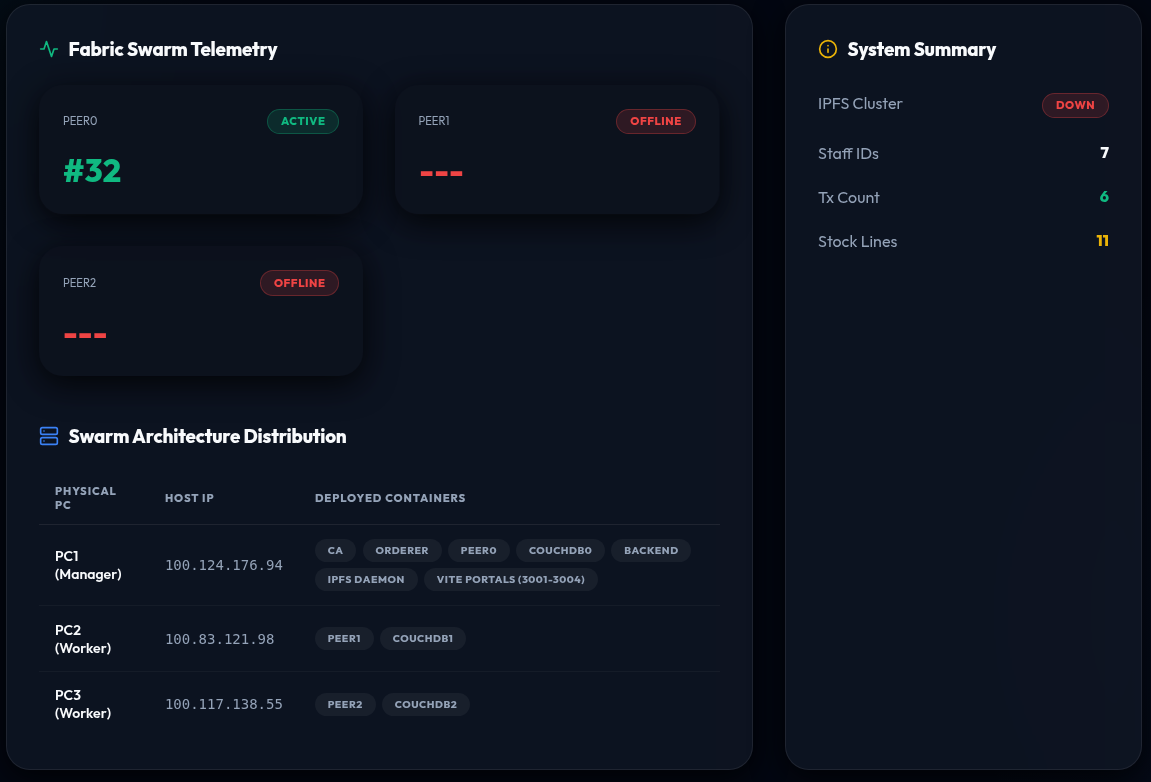
\includegraphics[width=0.85\textwidth]{ankit_dashboard.png}
    \begin{itemize}
        \item \textbf{Description:} High-level governance interface for hospital administrators to oversee all system modules and network status.
    \end{itemize}
\end{frame}

\begin{frame}{Workforce Registry (Ankit Chaudhari - 25CSM2R03)}
    \centering
    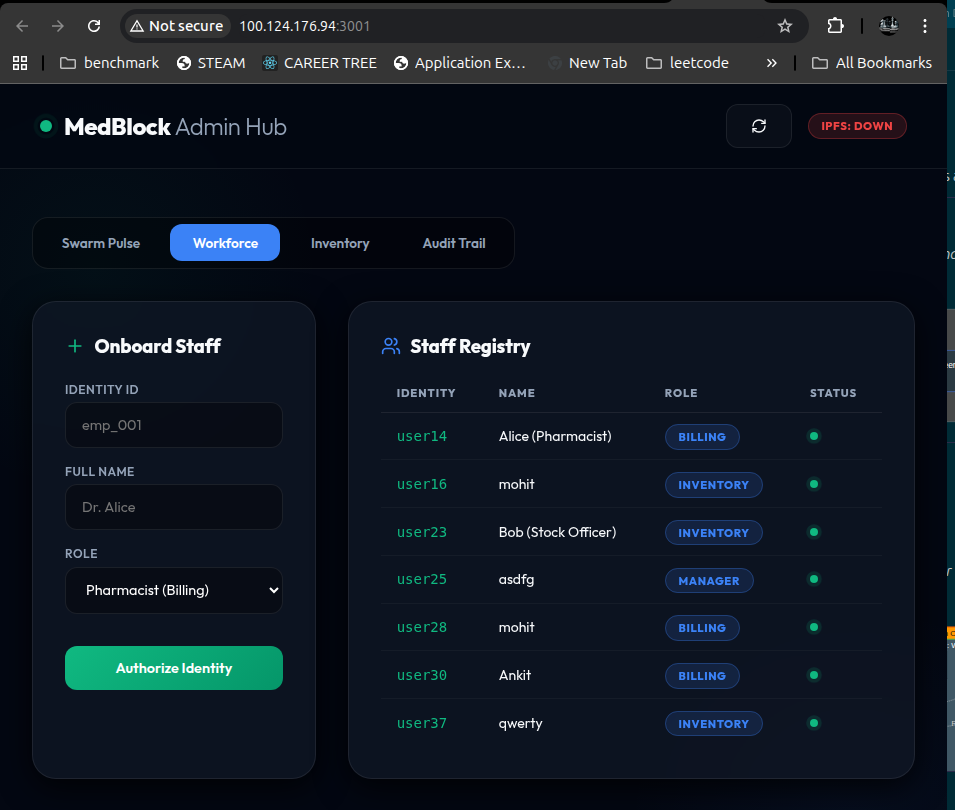
\includegraphics[width=0.85\textwidth]{ankit_workforce.png}
    \begin{itemize}
        \item \textbf{Description:} Employee enrollment interface. Assigns roles (Doctor, Pharmacist, Inventory) and provisions cryptographic identities.
    \end{itemize}
\end{frame}

\begin{frame}{Network Monitoring (Ankit Chaudhari - 25CSM2R03)}
    \centering
    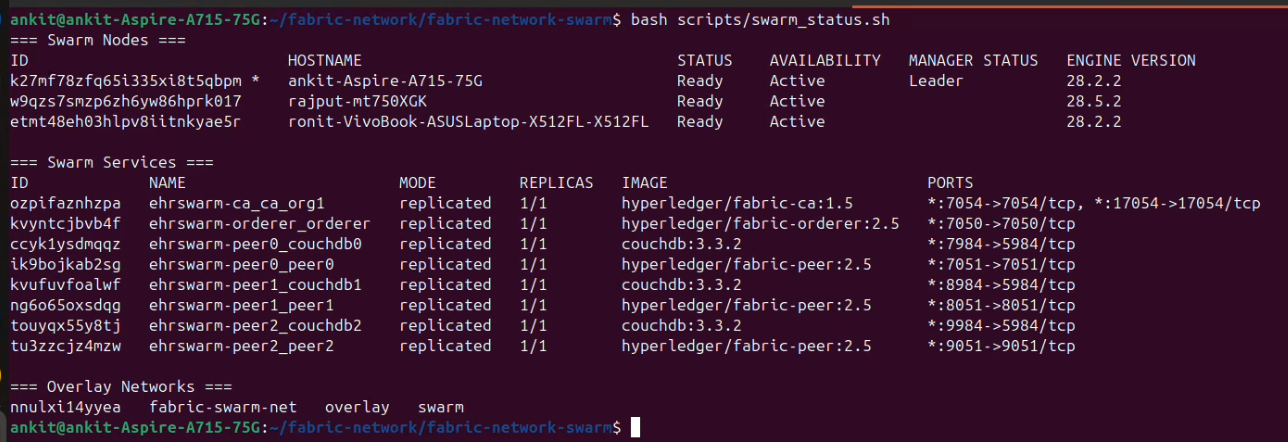
\includegraphics[width=0.85\textwidth]{ankit_status.png}
    \begin{itemize}
        \item \textbf{Description:} Real-time visualization of Swarm node health, block height, and Gossip synchronization status.
    \end{itemize}
\end{frame}

\begin{frame}{Blockchain Audit Trail (Ankit Chaudhari - 25CSM2R03)}
    \centering
    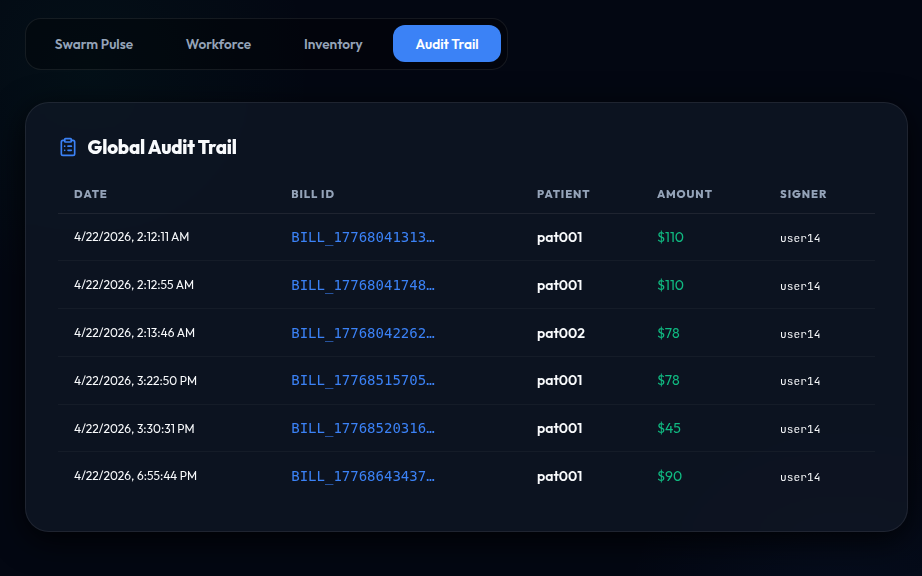
\includegraphics[width=0.85\textwidth]{ankit_audit.png}
    \begin{itemize}
        \item \textbf{Description:} Transparent record of all activities on the ledger, allowing managers to pull global hospital records for oversight.
    \end{itemize}
\end{frame}

\begin{frame}{Inventory Oversight (Ankit Chaudhari - 25CSM2R03)}
    \centering
    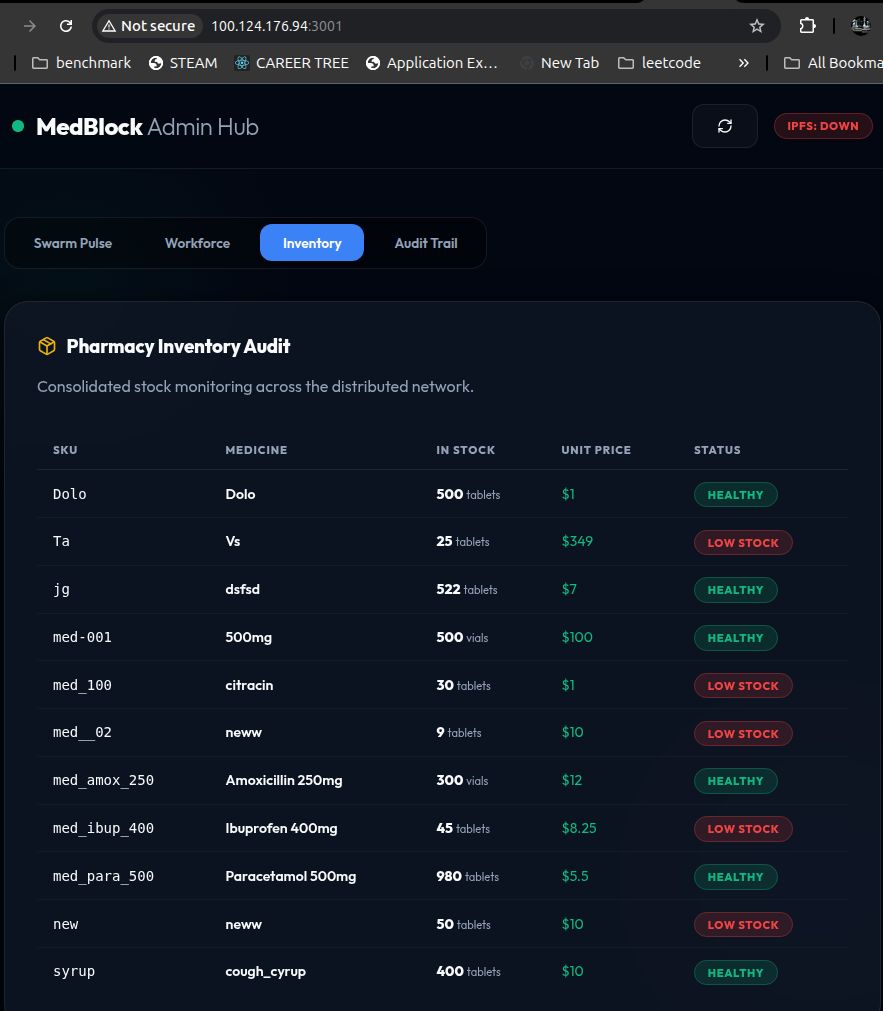
\includegraphics[width=0.85\textwidth]{ankit_inventory.png}
    \begin{itemize}
        \item \textbf{Description:} Read-only view of global stock levels across all modules, ensuring transparency in medicine supply.
    \end{itemize}
\end{frame}

% --- MOHIT ---
\subsection{Mohit Tomar}
\begin{frame}{Smart Contract Lead: Mohit Tomar (25CSM2R13)}
    \begin{block}{Role \& Responsibility}
        Development of Node.js Chaincode, CouchDB Rich Queries, and clinical portals (Patient \& Pharmacist).
    \end{block}
    \begin{itemize}
        \item \textbf{Containers Hosted on PC2:} Peer1, CouchDB1, Patient Portal, Pharmacist Portal.
        \item \textbf{Key Highlights:} Identity Resolution algorithm, attribute-based access control, and IPFS anchoring logic.
    \end{itemize}
\end{frame}

\begin{frame}{Patient Portal (Mohit Tomar - 25CSM2R13)}
    \centering
    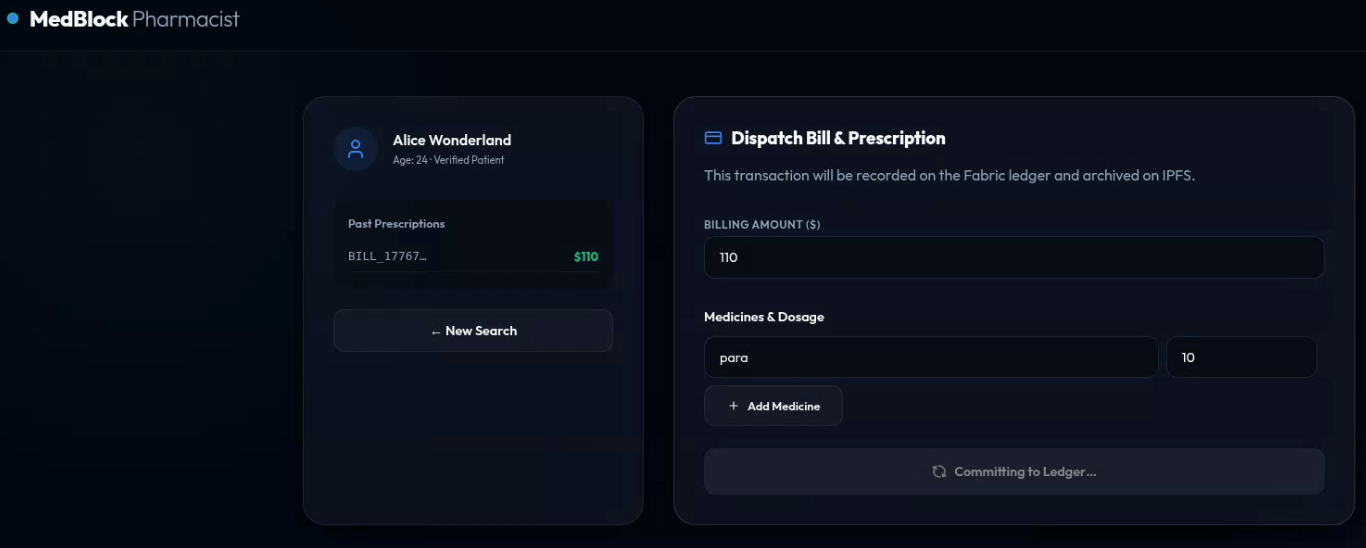
\includegraphics[width=0.85\textwidth]{mohit_pat_portal.png}
    \begin{itemize}
        \item \textbf{Description:} Self-Sovereign Identity portal where patients can view medical history and manage record access.
    \end{itemize}
\end{frame}

\begin{frame}{Pharmacist Portal (Mohit Tomar - 25CSM2R13)}
    \centering
    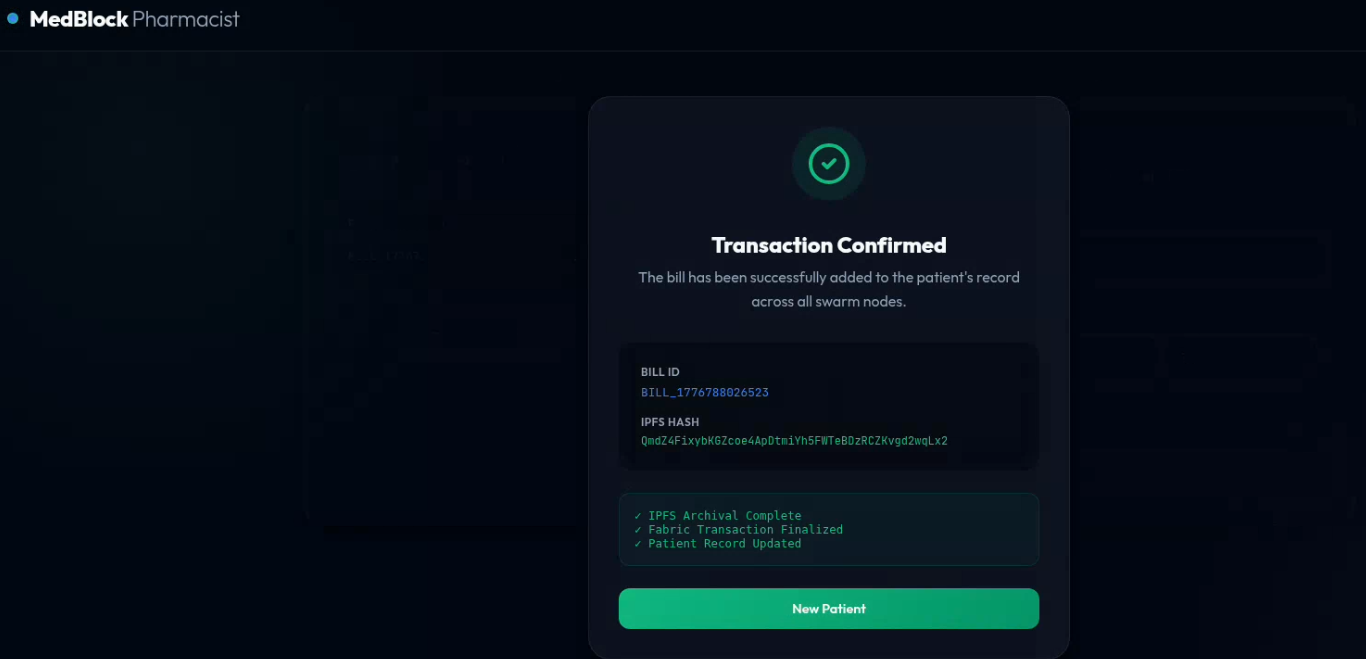
\includegraphics[width=0.85\textwidth]{mohit_pharm_portal.png}
    \begin{itemize}
        \item \textbf{Description:} Billing and prescription fulfillment interface using ABAC to ensure data privacy.
    \end{itemize}
\end{frame}

% --- RONIT ---
\subsection{Ronitsingh Rawat}
\begin{frame}{API Gateway Architect: Ronitsingh Rawat (25CSM2S06)}
    \begin{block}{Role \& Responsibility}
        Central API Gateway (Node.js SDK), Wallet Management, and Inventory Supply Chain Application.
    \end{block}
    \begin{itemize}
        \item \textbf{Containers Hosted on PC3:} Peer2 (Redundancy), CouchDB2, API Gateway, Inventory Portal.
        \item \textbf{Key Highlights:} Smart Routing algorithm, deterministic certificate mapping, and high availability setup.
    \end{itemize}
\end{frame}

\begin{frame}{Inventory Supply Chain (Ronitsingh Rawat - 25CSM2S06)}
    \centering
    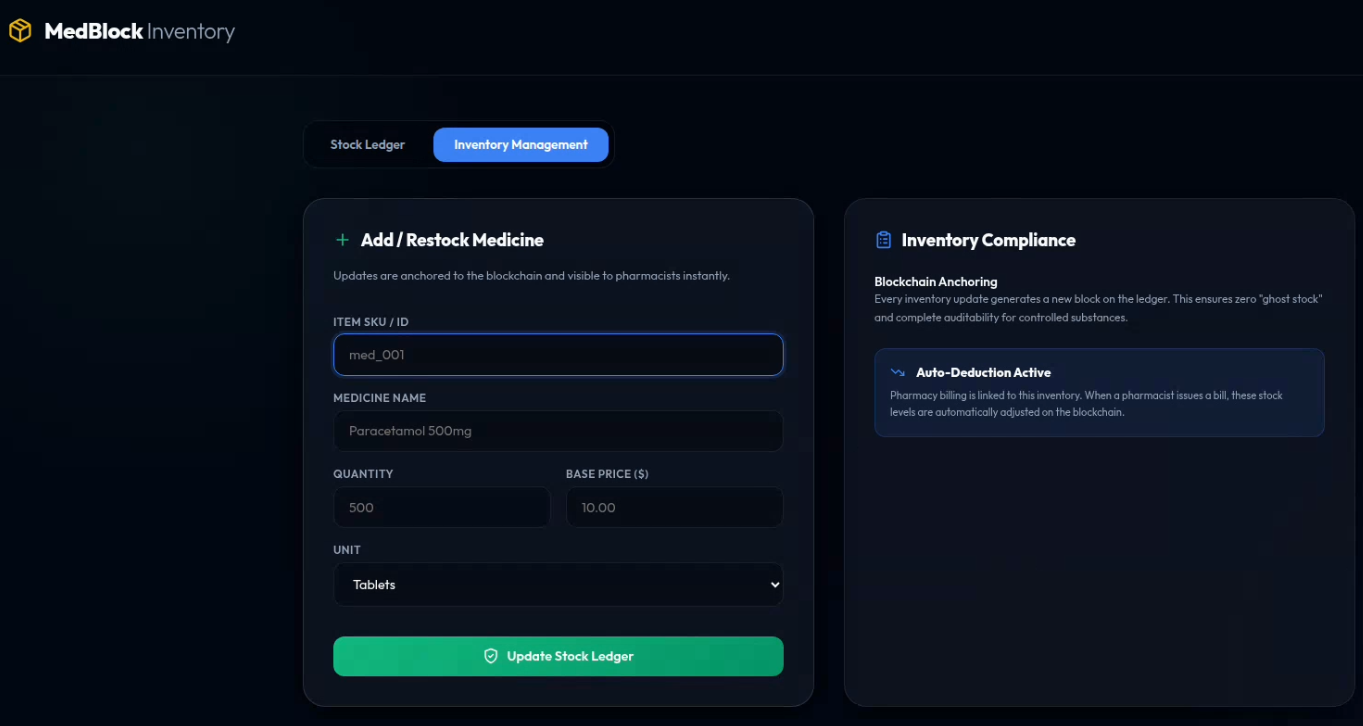
\includegraphics[width=0.85\textwidth]{ronit_inv_portal1.png}
    \begin{itemize}
        \item \textbf{Description:} Entry point for adding new medicine stock to the blockchain ledger with immutable timestamps.
    \end{itemize}
\end{frame}

\begin{frame}{Stock Management (Ronitsingh Rawat - 25CSM2S06)}
    \centering
    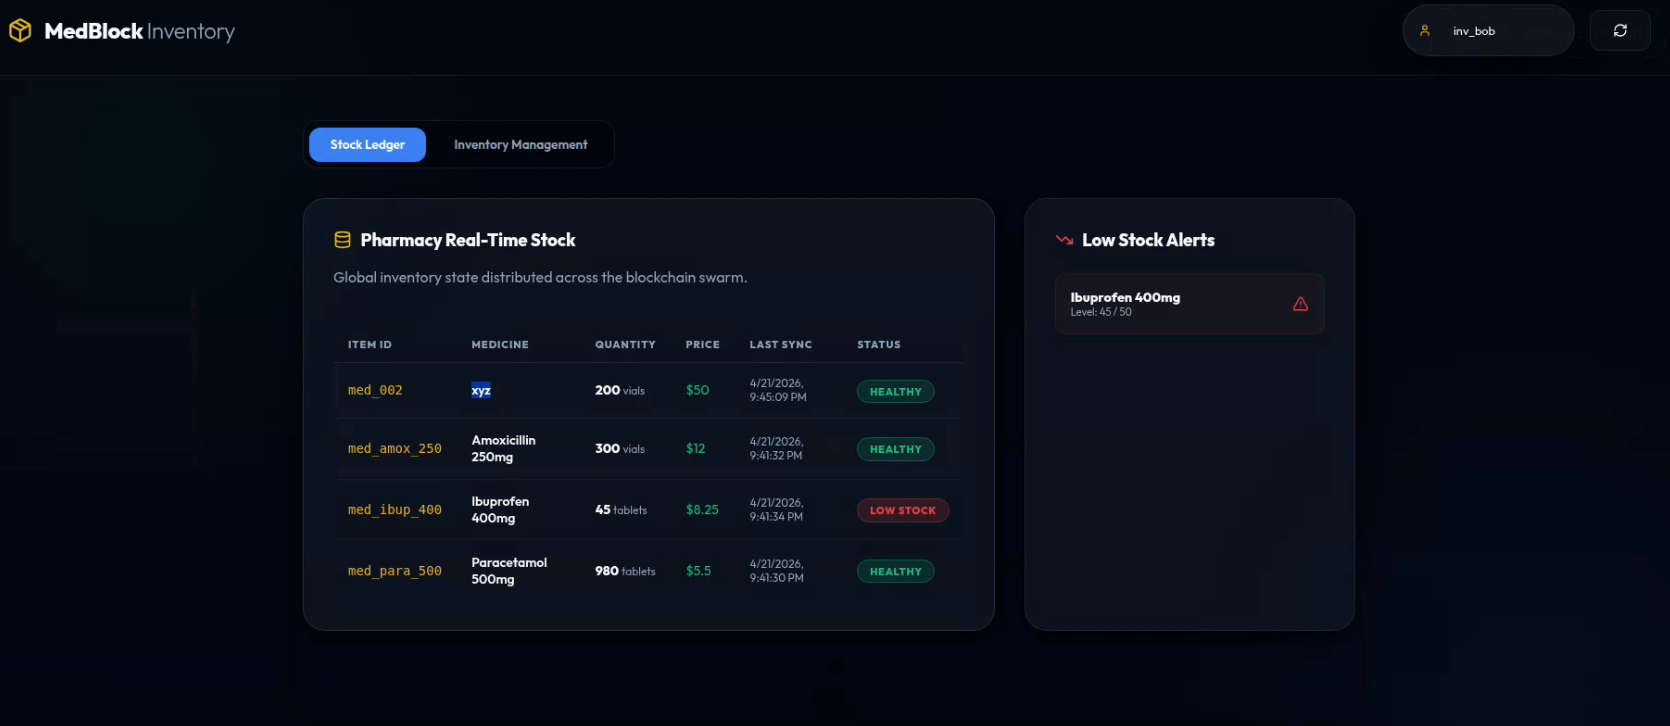
\includegraphics[width=0.85\textwidth]{ronit_inv_portal2.png}
    \begin{itemize}
        \item \textbf{Description:} Managing existing stocks and tracking deductions, linked atomically to the billing module.
    \end{itemize}
\end{frame}

\section{Verification}
\begin{frame}{Network Verification}
    \begin{itemize}
        \item \textbf{Ledger Sync:} All three peers (Peer0, Peer1, Peer2) reported identical block heights and matching hash values.
        \item \textbf{State Replication:} CouchDB instances on all nodes show synchronized world state.
        \item \textbf{Fault Tolerance:} Verified by taking one peer offline (PC2) and routing transactions through the redundant node (PC3).
    \end{itemize}
\end{frame}

\section{Conclusion}
\begin{frame}{Conclusion}
    \begin{enumerate}
        \item Successfully implemented a distributed EHR system across multiple physical nodes.
        \item Achieved perfect data consistency via Hyperledger Fabric's Gossip protocol.
        \item Ensured security and privacy through ABAC and X.509 digital identities.
        \item Built functional clinical, administrative, and inventory portals.
    \end{enumerate}
\end{frame}

\begin{frame}
    \centering
    \Huge Thank You! \\
    \vspace{20pt}
    \Large Questions?
\end{frame}

\end{document}
